\textbf{Consider the nonlinear initial value problem
\begin{align*}
u_t=u_{xx}+e^u,~~~~x\in [-1,1],~~t>0,~~u(\pm 1,t)=u(x,0)=0,
\end{align*}
for the unknown function $u(x,t)$. To at least eight digits of accuracy, what is $u(0,3.5)$, and what is the time $t_5$ such that $u(0,t_5)=5$.
}
\newline

The numerical scheme used in this problem is the following,
\begin{align*}
u^{n+1}=u^{n}+\Delta t\left[Du^{n}+e^{u^{n}}\right].
\end{align*}
We have obtained the solutions shown in figure 4 and the following results,
\begin{align*}
t_5&=3.53594879,\\
u(0,3.5)&=3.53878310.
\end{align*}

It is evident given the results that the solutions starts developing slowly but, because of the exponential non-linear term, it accelerates quickly. This can be appreciated by realizing that it takes the solution $t=3.5$ to reach the red curve, and only $t_5-3.5 = 0.03594879$ to get to the blue curve.

\begin{figure}[H]
\centering
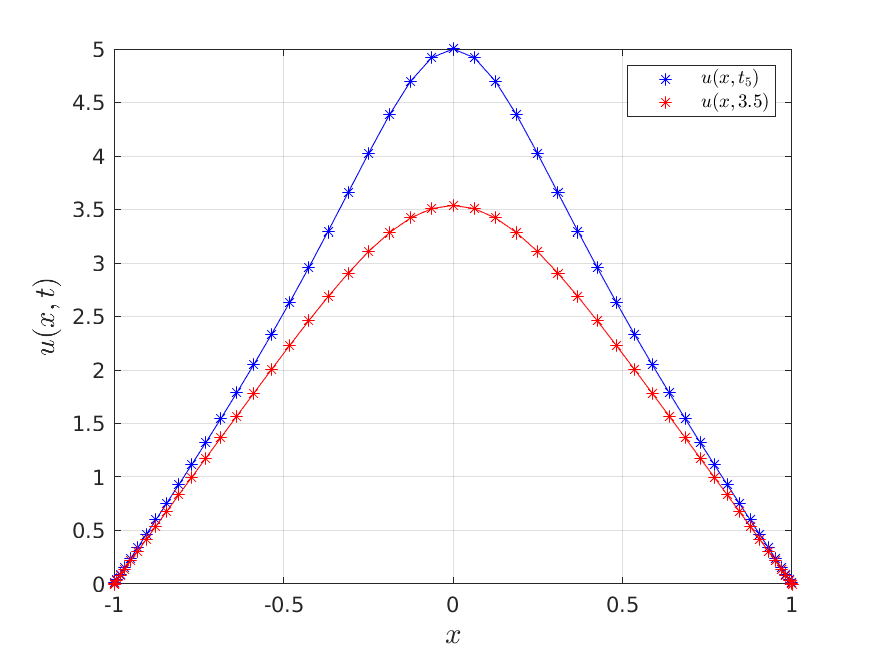
\includegraphics[scale=0.9]{P3.png}\caption{Numerical solution of the non-linear PDE at $t=3.5$ and at $t_5$, time when $u(0)=5$.}
\end{figure}

\subsection*{Matlab code for this problem}
\begin{verbatim}
%% Homework 4, Problem 3 - Francisco Castillo'
clear all; close all; clc;
labelfontsize = 14;
linewidth = 2;

N = 50;
dt = 8e-1/N^3;
[D,x] = cheb(N); % D:(N+1)x(N+1), x:(N+1)x1
x = x(2:N);
D2=D^2;
D2 = D2(2:N,2:N);
u = zeros(size(x));
u35 = u;
u0 = u(N/2);
tobs = [3.5 100];
t = 0;
k=1;
igraph = 1000;
tstep = 0;

while u0<5
    if (t+dt>tobs(k))
        dt=tobs(k)-t;
        t=t+dt;
        k=k+1;
    else
        t=t+dt;
        dt = 8e-1/N^3;
    end

    u = u +dt*(D2*u+exp(u));
    u0 = u(N/2);
    tstep = tstep+1;
    if t == tobs(1)
        u35 = u;
    end
    if (mod(tstep,igraph)==0 || round(u0,10)>=5)
        h1 = plot([1;x;-1],[0;u;0],'b*');
        hold on
        plot([1;x;-1],[0;u;0],'b')
        if (u35~=0)
            h2 = plot([1;x;-1],[0;u35;0],'r*');
            plot([1;x;-1],[0;u35;0],'r')
        end
        grid on
        axis([-1 1 0 5])
        xlabel('$x$','interpreter','latex','fontsize',labelfontsize)
        ylabel('$u(x,t)$','interpreter','latex','fontsize',labelfontsize)
        hold off
        shg
    end
end
legend([h1 h2],'$u(x,t_5)$', '$u(x,3.5)$','interpreter','latex')
saveas(gcf,'Latex/FIGURES/P3','png')
\end{verbatim}